\documentclass[12pt]{article}
\usepackage{macros}
\usepackage{bbm}
\usepackage{longtable}
\usepackage{titlesec}
\singlespacing


\titleformat{\section}
  {\normalfont\sffamily\Large\bfseries}
  {\thesection}{.5em}{}
\titleformat{\subsection}
  {\normalfont\sffamily\large\bfseries}
  {\thesubsection}{.5em}{}
  
\titleformat{\subsubsection}
  {\normalfont\sffamily\normalsize\bfseries}
  {\thesubsubsection}{.5em}{}
  
\newcommand{\cm}{{\color{Red}{\textsf{[C]}}}}
\newcommand{\one}{\mathbbm{1}}
\newcommand{\logit}{\operatorname{logit}}
\hypersetup{urlcolor=Purple}

% \singlespacing
\newgeometry{margin=1in}
\pagestyle{fancy}
\rhead{\textsf{J.~Chen and J.~H.~Yang}}
\lhead{\textsf{Stat 195}}
\chead{\textsf{\bfseries An Election Prediction Post-mortem}}


\title{\vspace{-1.5cm}\sffamily\bfseries{An Election Prediction Post-mortem}}
\author{\vspace{-.5cm}Jiafeng Chen \and Joon Hyuk Yang\thanks{The authors thank Lucas Janson, Zhirui Hu, and Dongming Huang for helpful comments on an earlier draft. We shall address a number of comments in this report, which shall be denoted with the symbol \cm.}}
\begin{document}
\maketitle
% \tableofcontents
\section{Our model}
\label{sec:intro}

In this section, we provide a quick review of our model. Let \begin{equation}
  Y_i = \frac{\text{Republican\%}}{\text{Republican\%}+\text{Democrat\%}}
  \label{eq:def_y}
\end{equation}
be the outcome variable of interest, where $i$ denote a district in a particular election. For $Y$ being a $435$-vector\footnote{In practice, we exclude the uncompetitive races from $Y$.} representing elections in 2018, we form a linear probability prior\footnote{\cm{} Zhirui has a comment that even though $Y_i$ is approxiately Normal by the CLT, the underlying proportion $p$ could still have a non-Normal distribution ($p$ is random from a Bayesian perspective). The response is that we care about the distribution of $Y_i$, since it determines the winner, while the true proportion $p$ does not.} \begin{equation}
  Y \sim \Norm(\mu_0, \Sigma_0)\label{eq:first}
\end{equation}
where $\mu_0 = X\beta_0, \Sigma_0$ is estimated
on the training data. To estimate $\beta_0$ and $\Sigma_0$ in \eqref{eq:first}, we use a cross-validated elastic net for $\beta_0$; this yields $\epsilon = Y_{\text{tr}} - \hat \mu_0^{\text{tr}}$ on the training set. We consider two formats for $\Sigma_0$. With \emph{diagonal} restriction, we simply let 
\begin{equation}
  \hat {\Sigma_0}_{ii} = \frac{1}{n_i} \sum_{j : i\in\text{state}(j)} \epsilon_j^2 = \sum_j \frac{\one\pr{i\in\text{state}(j)}}{\sum_{j'} \one\pr{i\in\text{state}(j')}} \epsilon_j^2, \qquad n_i = |\{j : i\in\text{state}(j)\}|
\label{eq:diag_var}
\end{equation}
be a state-smoothed estimate of variance on the training data. With \emph{unrestricted} $\Sigma_0$, consider the vectors $\epsilon_{(i)}$ being $\epsilon$ entries corresponding to districts with the same label (e.g. AL--01) as $i$,\footnote{Due to redistricting, the entries in $\epsilon_{(i)}$ could be completely unrelated to district $i$ in 2018.} indexed by time. We compute\footnote{\cm{} The corresponding procedure in the original report is incorrect due to a computational error in the following expression---we did not raise the variance terms to $1/2$-power in computing the off-diagonal covariance entries. As a result, the off-diagonal entries are small in our original report, and the resulting predictions are extremely similar. This is no longer the case once we correctly implemented \eqref{eq:unres_var}---see an email to Zhirui Hu on election day regarding this issue.} \begin{equation}
  \hat{\Sigma_0}_{ij} = \kappa \hat \rho_{ij} \pr{\hat {\Sigma_0}_{ii} \hat {\Sigma_0}_{jj}}^{1/2},\, i\neq j,\quad \hat \rho_{ij} = \hat{\corr}(\epsilon_{(i)}, \epsilon_{(j)}), \quad \kappa\in [0,1]
\label{eq:unres_var}
\end{equation}
where $\hat{\corr}$ denotes the empirical correlation operator and $\kappa$ is a shrinkage factor chosen so that the resulting estimate of $\Sigma_0$ is positive-definite. We assume that a poll outcome $Z_j$ has a normal distribution conditional on $Y$: $Z_j \mid Y \sim \Norm(a_{Z_j}^T Y, \sigma_{Z_j}^2)$, where $a_{Z_j}$ and $\sigma_{Z_j}^2$ are specified in our orginal report. This allows us to update the prior in \eqref{eq:first} and arrive at a posterior \begin{equation}
  Y \mid Z \sim \Norm(\mu, \Sigma),
  \label{eq:post}
\end{equation}
from which we generate our predictions by drawing from the posterior \eqref{eq:post}. The final predictions of the two models, diagonal and unconstrained, are plotted in \Cref{fig:model}.\footnote{\cm{} There was a comment regarding where the empty bars in the histograms in \Cref{fig:model} come from. We are calling the \texttt{seaborn.distplot} library function in Python. The data being plotted are integers, and so if the bin-size of the histogram is not integral, then we might see empty bins. }
\begin{figure}[tb]
  \centering
  \includegraphics[width=.7\textwidth]{rep_seats_with_diagonal_prior.pdf}
  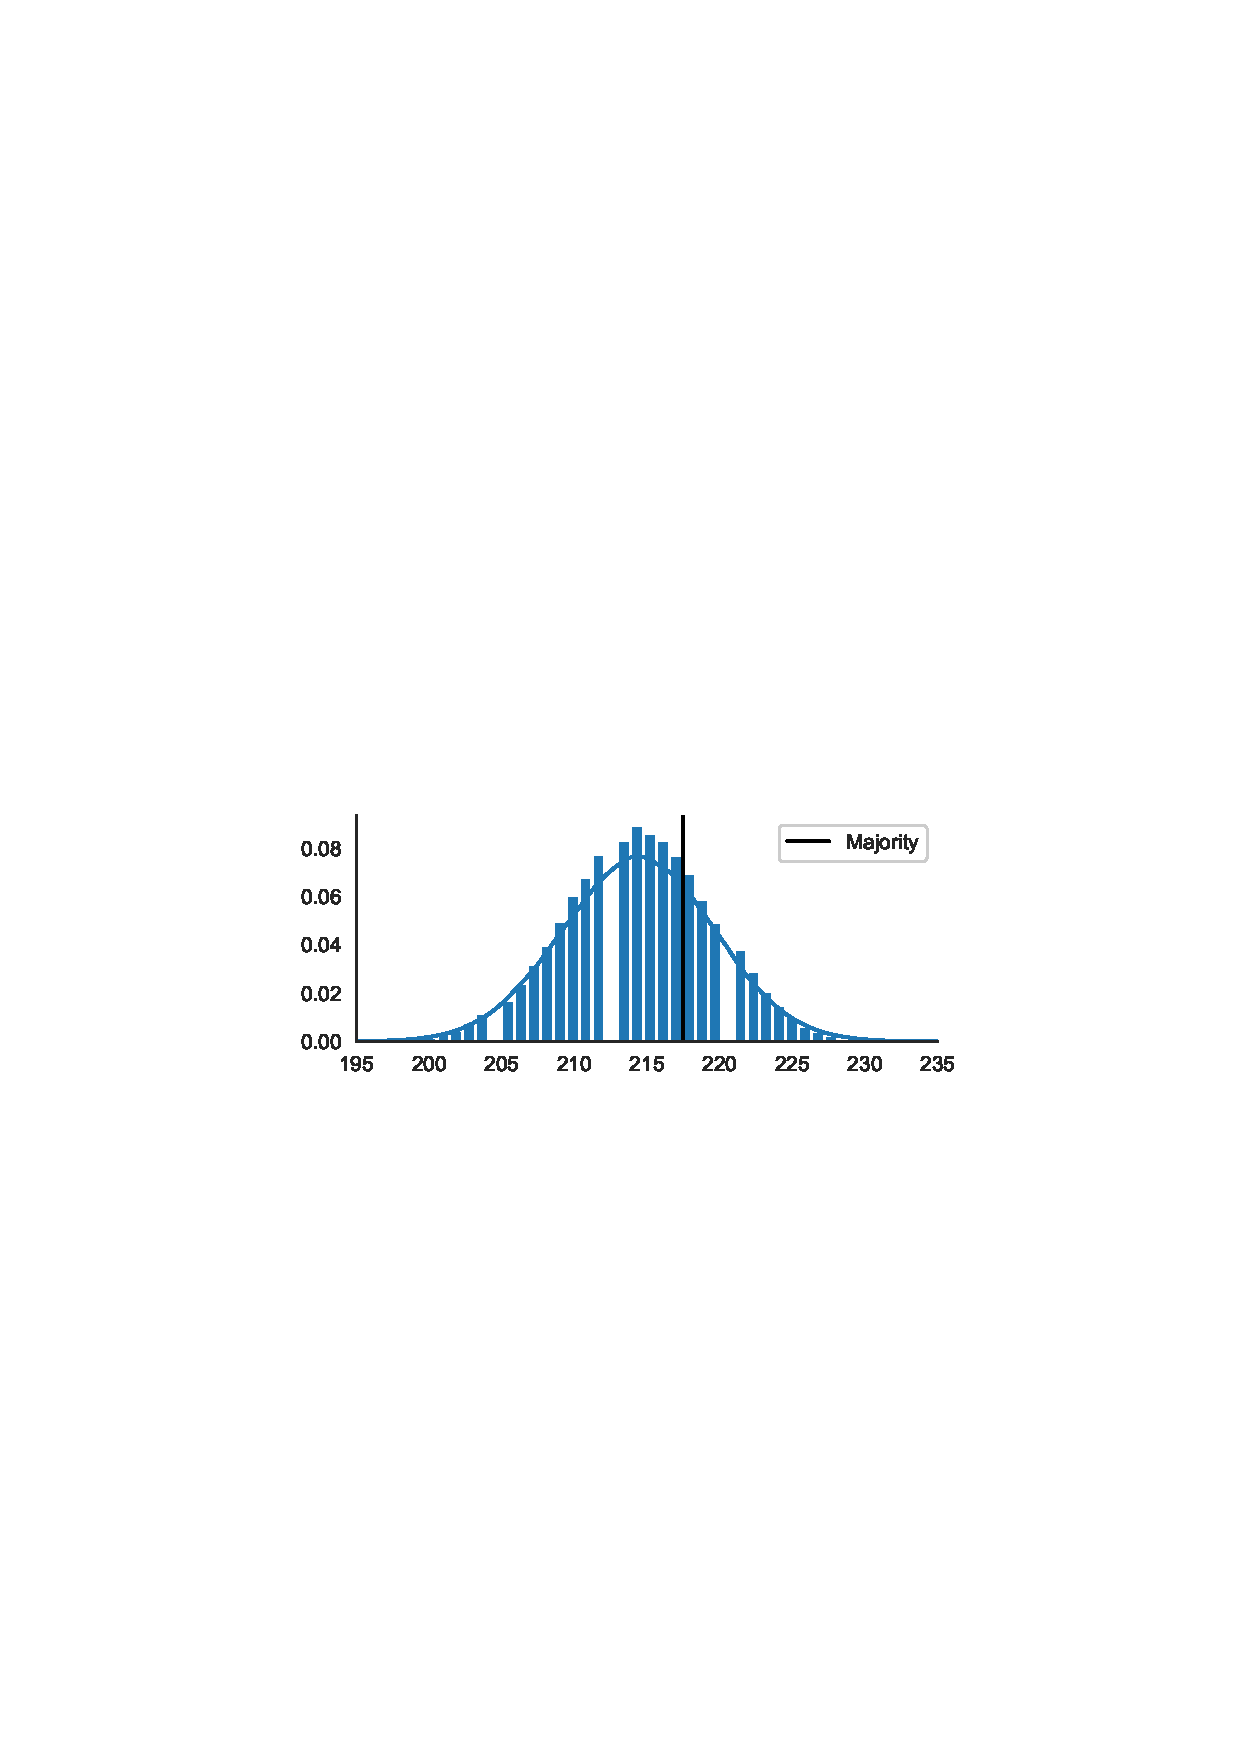
\includegraphics[width=.7\textwidth]{rep_seats.pdf}
  \caption{Model predictions. Top: diagonal. Bottom: unconstrained. }
  \label{fig:model}
\end{figure}

The rest of this report is organized as follows. \Cref{sec:overview} gives an overview of our prediction quality compared to the FiveThirtyEight benchmark. \Cref{sec:mu,sec:sigma,sec:polls} discusses issues and methods in fitting $\mu_0$, $\Sigma_0$, and the polling data, respectively. \Cref{sec:conc} concludes.

\section{Overview of prediction quality}
\label{sec:overview}
We plot a comparison of prediction quality between our prediction and that of FiveThirtyEight, broadly considered to be the state-of-the-art.\footnote{We take the latest prediction for each district generated by FiveThirtyEight's house model (\url{https://projects.fivethirtyeight.com/2018-midterm-election-forecast/house/}, and transform the prediction into a statistic that corresponds to \eqref{eq:def_y}.} The $R^2$ by regressing actual vote share on predicted vote share             and a constant for the diagonal model, unconstrained model, and FiveThirtyEight's            model is $0.897$, $0.893$, and $0.967$, respectively.% \Cref{tab:res} shows the number of correctly called races by model and winning party. Both \Cref{fig:quality,tab:res} show that the diagonal model performs better than the unconstrained model, and that both underperform relative to FiveThirtyEight's model. Moreover, \Cref{tab:res} shows that all three models underestimated the Democrats' performance in the midterm elections, while the diagonal outperforms unconstrained, and both of our models underperform that of FiveThirtyEight's.
\begin{figure}[tb]
  \centering
  \includegraphics{prediction_quality.pdf}
  \caption{Quality of our prediction compared to that of FiveThirtyEight. The point that all predictions incurred large positive residuals is Alaska's district-at-large, where the Republican won a competitive race, yet the Republican's opponent is an Independent and not a Democrat. Thus \eqref{eq:def_y} would define the response variable being 1, even though the race is fairly competitive.}
  \label{fig:quality}
\end{figure}
\begin{table}[tb]
  \caption{Number of correctly called races for each model by winning party of each district (top pane), and number of expected seats won by Democrats compared to ground truth (bottom pane).}
  \label{tab:res}
  \vspace{.4em}
  \centering
\begin{tabular}{lllll}
\toprule
{} & Total & Diagonal correct & Unconstrained correct & 538 correct \\
Winner                             &       &                  &                       &             \\
\midrule
Democrat                           &   240 &              216 &                   211 &         226 \\
Republican                         &   195 &              190 &                   187 &         193 \\
\midrule Expected Democratic Seats &   240 &              225 &                   223 &         233 \\
\bottomrule
\end{tabular}

\end{table}

It is clear from \Cref{tab:res,fig:model,fig:quality} that the unconstrained model suffers from too little precision, as the correlation operator in \eqref{eq:unres_var} is extremely noisy,\footnote{As Zhirui's comment \cm{} pointed out.} since the correlation is only taken over the four election years from 2010--2016. The unconstrained model was motivated by the fear that without modeling correlation of elections, the prediction model is going to be overly precise and would overlook systemic polling and modeling errors as was the case with the 2016 presidential election. However, it does seem that modeling correlation in the manner of \eqref{eq:unres_var} is not a good idea. From this point, we only consider the diagonal model. 

% \begin{figure}[tb]
%   \centering
%   \includegraphics{likelihood_dist.pdf}
%   \caption{The distribution of log likelihood over data generated from the fitted diagonal model.}
%   \label{fig:likelihood}
% \end{figure}

The benefit of explicit probabilistic modeling in the manner that we have done
is that we can evaluate the likelihood of the outcome that materialized. 
Consider the the distribution of the likelihood $\log L(\tilde Y)$ of data $\tilde Y \sim \Norm(\mu, \Sigma)$ generated under our model-fitted posterior. The 0.1\%-percentile of the likelihood is $630.35$. With the general intuition of hypothesis testing, we reject the model if the observed data has extremely low likelihood under the model. Evaluating the data transformed via \eqref{eq:def_y} suffers from extraordinarily low likelihood of a few observations, due to the presence of Independents (as in the caption of \Cref{fig:quality}). However, even with untransformed data, the data-likelihood is still exceptionally low compared to the purported data-generating distribution:
The log-likelihood of transformed data (as in \eqref{eq:def_y}) is 41.75, while the log-likelihood of untransformed Republican vote share is 442.25.%

The reason of the low likelihood seem to be that the variance of the model being too low, as $\mu$ is fairly close to the materialized outcome, by \Cref{fig:quality}. We can consider a variance inflation parameter $\sigma^2$ which maximizes the data likelihood under model $\Norm(\mu, \sigma^2 \Sigma)$. The fitted $\sigma^2$ is 4.262 for transformed data and 2.224 for untransformed data. Both estimates would strongly reject a null hypothesis of $\sigma^2 =1$.

\section{Fitting $\mu_0$}
\label{sec:mu}

\subsection{Data and Preprocessing}

Much of the data that we collected are of limited reliability. For instance, the gender of the candidiate, upon manual inspection, was wrong in many cases. We used a Python \texttt{gender-guesser} library to account for this while marking gender neutral names as 0.5. 

Data reliability issues imply that (1) we could have improved our data cleaning
process by looking up each candidate and filling in inconclusive entries, and
(2) features such as presidential approval or education level may have suffered
from inaccurate data reporting or exhibit high variance by being a point
estimate as opposed to an aggregate over surveys from longer periods of time.

In Part I, we also discussed the effectiveness of Google Trends's relative
popularity of search queries. However, there were several assumptions made that
may have proved problematic. First, search frequency is a good proxy
for interest, but it does not translate to support. We can imagine various
scenarios such as an incumbent candidate not having as many search queries by
virtue of already being well-known, or having a much higher search query due to
a negative press release. As our model relies on a linear model with at most a
second degree basis transform, tracing complex, non-linear relationships was
limited without introducing overfitting. Second, for certain
states (especially those with a low population), acquiring search frequency
ratio of candidate names at a State-level granularity was impossible because a
lack of absolute number of queries. We imputed these ratios with the ratios of a
nation-wide search, which might introduce bias, as there are more people living in blue states than in red states. Last and not least, even for states
where there are enough queries to return a state-level ratio, such as in Alaska
(\Cref{fig:candidate_only}), the resulting ratio alone may not be a discerning
indicator for candidate preference.

\begin{figure}[tb]
  \centering
  \includegraphics[scale=0.4]{alaska_candidate}
  \caption{Google Trends search frequency ratio of Democratic vs. Republican candidate in Alaska at large.}
  \label{fig:candidate_only}
\end{figure}

A better approach to utilizing Google Trends data would be to have a list of key issues by party from institutional knowledge or from analyses of party platforms, and compare the interest of Republican flagship issues against Democratic ones.\footnote{This approach would require some heavy topic/language modeling techniques in machine learning just to collect the data.} For instance, \Cref{fig:trends_issues} shows the Google Trends frequency results for four key issues: guns, defense, healthcare, and wellness. The first two are the flagship areas in which Alaska's Republican candidate emphasized, while the latter two are those prioritized by the Democratic candidate. The overall running average of these issues in Alaska suggests that there is ample room to augment our data by feeding in a more holistic picture of search query frequency ratios on topics that are brought forth by candidates.~Don Young, the Republican,~took Alaska's seat at the~House.

\begin{figure}[tb]
  \centering
  \includegraphics[scale=0.4]{trends_issues}
  \caption{Google Trends search frequency ratio in Alaska on guns, healthcare, defense, and wellness. On average, guns are more frequently queried compared to healthcare, and defense more frequently than wellness.}
  \label{fig:trends_issues}
\end{figure}

\subsection{Covariate and model selection in forming prior}

We examine the effect of covariate selection by running the procedure while
leaving one of the covariates out, somewhat mimicking a backward stepwise model
selection procedure. Since the design matrix $X$ included both linear and
quadratic terms of the covariates, leaving one covariate out leaves out all its
quadratic terms. We present the $R^2$ of the regression of the 2018 data on the
predictions (as in \Cref{fig:quality}) in \Cref{tab:leave_out}. We see that
leaving out most covariates have little effect on the prediction quality, while
racial makeup, incumbency, and educational background are particularly important
for prediction. Moreover, for quite a few covariates, leaving them out actually
\emph{improves} fit, suggesting that the elastic net regularizer is not a
panacea for overfitting---in particular, if the covariates have little
predictive power, then in order for the regularizer to adequately control for
overfitting, it must have a high level of shrinkage, which may result in
underfitting, as the regularizer would discount variables that are highly
predictive.

We supplement the analysis in \Cref{tab:leave_out} with a calculation of Akaike and Bayesian information criteria for the elastic net fitting, as the $R^2$ on the 2018 data is not available at training time. In particular, we calculate the information criteria by computing\footnote{The degree-of-freedom calculation follows this talk by Hui Zou and Trevor Hastie on the elastic net: \url{https://web.stanford.edu/~hastie/TALKS/enet_talk.pdf}} \[
\hat {\mathsf{df}} = \tr\pr{X_A (X_A^T X_A + \lambda_2 I)^{-1} X_A^T}, \quad X_A = \text{active set of covariates $X$ under the LASSO},
\] 
We assume the likelihood is under the homoskedastic model $Y^i_{\text{tr}} \sim \Norm(X\beta, \sigma^2)$ and compute \begin{align*}
\mathsf{AIC} = 2 \pr{\hat {\mathsf{df}} - \sum_i \log 
L(Y_\text{tr}^i)} \qquad \mathsf{BIC} = 2 \pr{\hat {\mathsf{df}} \log N - \sum_i \log 
L(Y_\text{tr}^i) }.
\end{align*}
We show in \Cref{fig:ic_r2} that the information criteria roughly correlates to realized goodness-of-fit on the new data,\footnote{Better, i.e. lower, AIC/BIC values generally translates to higher $R^2$.} suggesting that model selection via AIC and BIC at training time can reduce generalization error. 

\begin{table}[tb]
  \caption{Effect on fit (among competitive races) of leaving one covariate (along with all higher-power terms that involve the covariate) out; we also show the performance of certain alternative prediction functions for $\mu_0$. \texttt{full} means full model. \texttt{quadratic} means leaving out all quadratic terms. \texttt{lasso\_select} means using a cross-validated LASSO to select covariates by discarding all covariates with zero fitted coefficent and running an elastic net on the rest of the covariates. \texttt{gradient\_boost} is a gradient boosting regression tree with validation-guided early stopping. \texttt{logit} is a model where $\mu_0 = X\beta_0$ is replaced with $\mu_0 = \logit^{-1}(X\beta_0)$---we fit an elastic net on $\logit$-transformed training data to obtain $\beta_0$. \texttt{kernel\_sigma} is the estimation procedure outlined in \Cref{sec:sigma}.}
  \label{tab:leave_out}
  \centering
  \vspace{.4em}
  \begin{tabular}{lllr}
\toprule
        Variable left out / Model name &  $R^2$ &       Variable left out / Model name &  $R^2$ \\
\midrule
         \texttt{minority\_percentage} & 0.7649 &  \texttt{same\_as\_pres\_party\_rep} & 0.8215 \\
               \texttt{rep\_incumbent} & 0.8062 &             \texttt{dem\_is\_female} & 0.8217 \\
 \texttt{percent\_bachelor\_or\_above} & 0.8086 &                \texttt{dem\_percent} & 0.8230 \\
              \texttt{gradient\_boost} & 0.8138 &             \texttt{rep\_is\_female} & 0.8235 \\
               \texttt{pres\_approval} & 0.8177 &               \texttt{lasso\_select} & 0.8238 \\
             \texttt{log\_med\_income} & 0.8182 &                       \texttt{logit} & 0.8259 \\
            \texttt{rep\_to\_tot\_oct} & 0.8183 &               \texttt{kernel\_sigma} & 0.8267 \\
            \texttt{rep\_to\_tot\_nov} & 0.8211 &              \texttt{dem\_incumbent} & 0.8272 \\
                         \texttt{full} & 0.8215 &                   \texttt{quadratic} & 0.8324 \\
                                       &        &  \texttt{same\_as\_pres\_party\_dem} & 0.8402 \\
\bottomrule
\end{tabular}

\end{table}

\begin{table}[tb]
  \caption{Effect on the information criteria of leaving one covariate out, along with all higher-power terms that involve the convariate. The table is sorted according to AIC.}
  \label{tab:ic}
  \centering
  \vspace{.4em}
  \begin{tabular}{lrrrr}
\toprule
{} &     $N$ & $\hat{\mathsf{df}}$ &      AIC &      BIC \\
\midrule
\texttt{pres\_approval}               &  $1530$ &               $161$ &  $-5269$ &  $-3217$ \\
\texttt{dem\_is\_female}              &  $1530$ &               $131$ &  $-5256$ &  $-3584$ \\
\texttt{rep\_is\_female}              &  $1530$ &               $156$ &  $-5245$ &  $-3256$ \\
\texttt{same\_as\_pres\_party\_rep}   &  $1530$ &               $149$ &  $-5237$ &  $-3337$ \\
\texttt{full}                         &  $1530$ &               $149$ &  $-5237$ &  $-3337$ \\
\texttt{rep\_to\_tot\_nov}            &  $1530$ &               $144$ &  $-5236$ &  $-3400$ \\
\texttt{dem\_percent}                 &  $1530$ &               $144$ &  $-5236$ &  $-3399$ \\
\texttt{same\_as\_pres\_party\_dem}   &  $1530$ &               $147$ &  $-5235$ &  $-3361$ \\
\texttt{rep\_to\_tot\_oct}            &  $1530$ &               $131$ &  $-5213$ &  $-3541$ \\
\texttt{log\_med\_income}             &  $1530$ &               $170$ &  $-5212$ &  $-3046$ \\
\texttt{percent\_bachelor\_or\_above} &  $1530$ &               $175$ &  $-5115$ &  $-2886$ \\
\texttt{rep\_incumbent}               &  $1530$ &               $179$ &  $-5002$ &  $-2725$ \\
\texttt{dem\_incumbent}               &  $1530$ &               $404$ &  $-4701$ &    $419$ \\
\texttt{minority\_percentage}         &  $1530$ &                $66$ &  $-4322$ &  $-3473$ \\
\bottomrule
\end{tabular}

\end{table}


\begin{figure}[tb]
  \centering
  \includegraphics{ic_rsq.pdf}
  \caption{Comparison between the information criteria in \Cref{tab:ic} and $R^2$ in \Cref{tab:leave_out}.}
  \label{fig:ic_r2}
\end{figure}

We also experiment with a some methods to improve model selection in \Cref{tab:leave_out}, treating the data from 2018 as a validation set. In particular, the \texttt{lasso\_select} entry in \Cref{tab:leave_out} represents a two-step procedure where a first-step LASSO regression is used to select covariates and a second-step elastic net is used to further control for overfitting and shrinkage. We see that this method marginally increases quality of fit. In \texttt{quadratic}, we simply leave out all quadratic terms in $X$, and rather discouragingly, this much sparser set of covariates perform better than both the \texttt{full} and the \texttt{lasso\_select} models. 

We also investigate whether alternative methods for fitting $\mu_0 =
f_\beta(X)$, for some functional form $f$ and parameters $\beta$, would have
done better. We fit a gradient boosting regression tree
(\texttt{gradient\_boost}) on the same input space as the original model
(\texttt{full}). We hold out a validation set and use an early stopping
rule---stopping when the validation error fails to improve for a number of
iterations.\footnote{We tried multiple hyperparameters for the early stopping;
all of them failed to generate better fit than \texttt{full}.}
\texttt{gradient\_boost} does not appear to have better fit than the elastic
net. We suspect that nonparametric methods like gradient boosting trees do not
utilize the rich probabilistic information in the input data,\footnote{the probabilistic
model \eqref{eq:first} fits fairly well by inspecting a Q--Q plot, despite the misspecification; see original
report for details} which results in a worse fit. This leads us to suspect that
better specified probabilistic models should do better. We correct for the
misspecification in \eqref{eq:first} by fitting $\beta$ on the logit-transformed
space of the original data, $
\logit(Y_\text{tr}) \sim \Norm(X_\text{tr}\beta_0, \Sigma_\text{tr}),
$
mimicking the \emph{logit-normal model} \cite[page 283]{agresti2015foundations}---so that the Normal distribution is properly specified on data that can take values in $\R$. However, modeling in the logit space does not lend well to the simple Bayesian updating in \eqref{eq:post} without using expensive MCMC simulations, and for convenience's sake, in prediction, we modify \eqref{eq:first} to $\Norm(\logit^{-1}(X\beta_0), \Sigma_0),$ which is again a slight misspecification.\footnote{Therefore, the \texttt{logit} model in \Cref{tab:leave_out} is not strictly-speaking a logit-normal model as in \cite{agresti2015foundations}---rather an ad hoc alternative inspired by the logit-normal model in the literature.} This model, \texttt{logit}, does appear to perform slightly better than the original model \texttt{full}, but the degree of improvement is probably too small to show meaningful conclusions.  


\section{Fitting $\Sigma_0$}
\label{sec:sigma}

The procedure outlined in \eqref{eq:diag_var} would provide downward-biased estimates of $\Sigma_0$, since we are using the \emph{fitted} residuals to estimate variance. An more ``honest'' \citep{athey2016recursive} approach for variance estimation would be to use a validation set. However, for the variance as in \eqref{eq:diag_var} to have any precision, each state in the validation set needs to include a substantial number of observations, which is difficult for states like Alaska or Montana. We consider an alternative approach in this section. Observe that \eqref{eq:diag_var} is a Nadaraya--Watson estimator where the kernel weighting is whether $i,j$ are from the same state. We can thus generalize \eqref{eq:diag_var} into 
\begin{equation}
  \hat {\Sigma_0}_{ii} = \sum_j \frac{K_h(x_j - x_i)}{\sum_{j'} K_h(x_j - x_i)}\epsilon_j^2
\label{eq:kernel_var}
\end{equation}
for some kernel function $K_h(x-x_0)$. \eqref{eq:kernel_var} codifies the
intuition that districts with similar observable characteristics should have
similar prediction error magnitudes, as in the intuition for FiveThirtyEight's
CANTOR model,\footnote{\url{https://fivethirtyeight.com/features/2018-house-forecast-methodology/}}
which uses a $k$NN kernel to identify similar districts. In the implementation demonstrated, we let
$K_h$ be the Gaussian kernel \[K_h(x-x_0) \propto
\exp\pr{-\frac{\norm{x-x_0}^2}{2h}},\] where $x, x_0$ are the \emph{linear}
terms comprising of all covariates used in \texttt{full}. We sum over $j$ that
are in a validation set, comprising of $10\%$ of observations selected at
random. The change in the prior variance $\Sigma_0$ have an impact on the
posterior $\mu$, since it changes the Bayesian updating. The impact of kernel
weighting in estimation of $\Sigma_0$ is also shown in \Cref{tab:leave_out}. We
see that the kernel weighting methods seem to increase quality of fit by a
minute amount, with relatively low sizes of bandwidth delivering better fits. 

We perform the same exercise at the end of \Cref{sec:overview} to check how far
the model under our posterior deviates from the data, and results are shown in \Cref{tab:kernel_res}.
\begin{table}[tb]
  \caption{Model evaluation of kernel-fitted $\Sigma_0$}
  \label{tab:kernel_res}
  \centering
  \vspace{.4em}
  \begin{tabular}{lrr}
\toprule
{} &  $h = .1$ &  $h = 1$ \\
\midrule
0.1\%-percentile Log Likelihood               &  575.9772 & 560.6451 \\
Data Log Likelihood (transformed)             &  185.7445 & 235.7885 \\
Data Log Likelihood (untransformed)           &  458.2238 & 507.2840 \\
Data-rationalizing $\sigma^2$ (transformed)   &    3.3033 &   2.9671 \\
Data-rationalizing $\sigma^2$ (untransformed) &    1.9167 &   1.5854 \\
\bottomrule
\end{tabular}

\end{table}
We see
that the kernel fitting alleviates, but does not eliminate, the problem of
overly sharp posterior variance discussed in \Cref{sec:overview}: The posterior
model is still sharply rejected by the data, but the inflation factor that the posterior
needs to rationalize the data is smaller with kernel smoothing of variance than
with our original model. Moreover, it appears that a higher degree of smoothing generates more agnosticism in the posterior, and therefore makes the posterior distribution contradict the data less. 

\section{Updating with polls}
\label{sec:polls}
We have seen from \Cref{sec:sigma} that our final estimates are still overly
precise, despite considerable efforts to more conservatively infer the prior
variance. Another reason for the rejection of our posterior model is
generalization error---the information contained in the training data are
2010--2016, which might not generalize to 2018, leaving bias in the prior
estimates (though \Cref{fig:quality} seems to suggest that this is not the
case). One way to reduce the generalization gap is to use polling information,
which encode the political environment in 2018 that we cannot have learned from
the 2010--2016 data. The Bayesian update \eqref{eq:post} also affects posterior
variance. In this section we consider alternative methods to deal with polling
data; however, due to time and resource constraints, we do not implement models considered in this section.

First, it has come to our attention that FiveThirtyEight does publish past
polling data, and thus the simplest way to incorporate polling data is to
construct covariates that take into account both recency and accuracy of polls.
Second, one large issue we faced is that the variance of polling results cannot
be explained by a simple Binomial likelihood. Our remedy in the previous report
is to approximate the Binomial likelihood with a Normal likelihood, with
variance inferred from the empirical variance of data. An alternative approach,
inspired by the problem of overdispersion in GLMs and quasi-likelihood
estimation \citep[][Chapter 8]{agresti2015foundations}, is to consider the
Binomial model as an exponential dispersion family model $p(y) =
\exp\pr{\frac{y\theta - b(\theta)}{\phi} + c(y, \phi)}$ with unknown dispersion
parameter $\phi$. For a given district, we can consider the \emph{maximum
quasi-likelihood estimate} (QMLE) \citep{agresti2015foundations} for the
Binomial parameter $p$ and its variance $\tau^2$ as a summary statistic of the
data, and use the QMLE to update the prior. Lastly, we are assuming that
conditional on $Y_i$, polls are independently distributed, which drastically
increase the influence of additional polls. However, one probably expects polls
to be correlated \cm{}. However, it is difficult to define or estimate
correlation among polls, since the polling data is not of a panel format. One
approach might be to consider some hyperparameter $\rho$ and correlation matrix
of the form $\corr(Z_i,Z_j) = \rho$.

As a further direction, due to the lack of polling in certain districts, we
could consider certain methods for imputing polling responses in unpolled
districts. For instance, suppose we observe individual-level data on, say,
browing history in a large number of districts, where some are polled and others
are not.~We can consider the individual as either a Democrat or a Republican, a
latent variable that we do not observe. However, polling gives the proportions
of Democrats and Republicans in some districts. One could build a model based on
the EM algorithm to infer the latent political leanings variable as a function
of observable individual-level data, as \cite{comarela2018browse} have
done.\footnote{For instance, if many individuals in a heavily Republican
district visit the website of Fox News regularly, we would learn that browsing
Fox News is correlated with being a Republican, even if we have no knowledge of
individual political leanings. We can then infer that an unpolled district in
which many people browse Fox News must lean Republican.} This model would then
be able to predict polling outcomes in unpolled districts by imputing the
political leanings of individuals observed in those districts. Of course, such a
method requires access to vast amounts of granular data, which we do not have.

\section{Discussion and conclusion}
\label{sec:conc}

We have considered modifications to all parts of our estimation procedure, outlined in \Cref{sec:intro}. We find in \Cref{sec:overview} that our procedure generally creates good point estimates, which are a bit less precise than the state-of-the-art; however, we also find that the posterior is too precise for the data to not reject the model, requiring an inflation factor of about two to four times to the variance in order for the model to not be rejected. We consider preprocessing, model selection, and feature selection in \Cref{sec:mu}; we consider a generalization of \eqref{eq:diag_var} and kernel methods to estimate variance in \Cref{sec:sigma}; and we sketch a few possible directions to improve the Bayesian updating.

\begin{comment}


Our prediction results rely heavily on the validity of our posterior update,
which is dominated by how informative we think the polling data is. However,
various polls are collected in several districts while none are conducted in
others. In fact, each pollster has such high variance that Nate Silver provides
pollster ratings, which Part I did not explicitly take into account. The
aggregate or \textit{overall} trend in polls is what Nate Silver explains as
being of greater interest.\footnote{Silver argues that both macro and micro
trends from polling data are important--the former being the aggregate poll
result and the latter being the pollster ratings. More information at
\url{fivethirtyeight.com/features/which-pollsters-to-trust-in-2018}} In order to
mitigate the noisy nature of polls and account for missing polls for districts,
we could introduce intermediate data between polls and~votes.

One such candidate could be people's browsing history, $B$, for each district.
Instead of solely relying on voting results to fit the parameters of $Z$, we can
regress over $B$ to predict the polling outcome $\tilde{Z}$. In turn, we can use
a kernel method to weigh various polls and even predict what polls would look
like in unpolled districts. By introducing the intermediate data, $B$ in this
case, we effectively \textit{hallucinate} polls that can be used to update our
posterior. Realistically we do not have labels for each individual browsing
history with a political affiliation, which means we must resort to techniques
such as the EM algorithm to estimate the maximum likelihood. More formally, we
can assume polling results as being a bimodal Gaussian mixture model such that
$Z = (1 - \Delta) \cdot Z_1 + \Delta \cdot Z_2$ where $Z_k \sim
\mathcal{N}(\mu_k, \Sigma_k)$ and Pr$(\Delta = 1) = \pi$. To approximate
$\theta_k = (\mu_k, \Sigma_k)$ for the densities $\phi_{\theta_k}(z)$, we repeat
the following \textit{Expectation} step \Cref{eq:expectation} and
\textit{Maximization} steps \Cref{eq:maximization1}, \Cref{eq:maximization2}
until convergence, such that

\begin{equation}
\hat{\gamma}_i = \frac{\hat{\pi}\phi_{\hat{\theta}_1}(z_i)}{\hat{\pi}\phi_{\hat{\theta}_1}(z_i) + (1-\hat{\pi})\phi_{\hat{\theta}_2}(z_i)} \text{\ ,} \qquad i = 1,2,\ldots, N
\label{eq:expectation}
\end{equation}

\begin{equation}
\hat{\mu}_k = \frac{\sum_{i=1}^{N}\{\hat{\gamma_i}^{I(k=1)} + (1-\hat{\gamma_i})^{I(k=2)}\}z_i}{\sum_{i=1}^{N}\{\hat{\gamma_i}^{I(k=1)} + (1-\hat{\gamma_i})^{I(k=2)}\}} \text{\ ,} \qquad k \in \{1,2\}
\label{eq:maximization1}
\end{equation}

\begin{equation}
\hat{\Sigma}_{1} = \frac{\sum_{i=1}^{N}\hat{\gamma}_i(z_i - \hat{\mu}_1)(z_i - \hat{\mu}_1)^T}{\sum_{i=1}^{N}\hat{\gamma}_i} \qquad \hat{\Sigma}_{2} = \frac{\sum_{i=1}^{N}(1-\hat{\gamma}_i)(z_i - \hat{\mu}_2)(z_i - \hat{\mu}_2)^T}{\sum_{i=1}^{N}(1-\hat{\gamma}_i)}
\label{eq:maximization2}
\end{equation}

where $\hat{\gamma}_i = \E(\Delta_i|\theta, Z)$ is the responsibility of, in this case, class 1 (e.g. Republican). Additionally, we must initialize the parameters $\theta = (\hat{\mu}_k, \hat{\Sigma}_k, \hat{\pi})$, which we can assign randomly with some  assumptions for better performance as illustrated in \cite{comarela2018browse}. Ultimately, by fitting data provided by Interet Service Providers against poll results, this method (\Cref{fig:browsing}) can be used to weigh various polls for a particular district as a Nadaraya-Watson kernel-weighted average, where the kernel $K_{\lambda}(\tilde{z}, z_i) = D(|z_i-\tilde{z}|/\lambda)$ and $D(t) = \phi(t)$. Furthermore, for districts without any polls, $\tilde{Z}_k \sim \mathcal{N}(\mu_k, \Sigma_k)$ can be used directly to proxy a poll by sampling from the density function.  

\begin{figure}[tb]
  \centering
  \includegraphics[scale=0.3]{browsing_diagram.pdf}
  \caption{Diagrammatic view of incorporating browsing history as an alternative to poll-based posterior update.}
  \label{fig:browsing}
\end{figure}

This is admittedly a roundabout way of calculating $\E(Y|Z,B)$. Although directly computing $\E(Y|B)$ may be attractive, often (including browsing history) it is difficult to find labeled data (political inclination), and even when using approximation algorithms, the number of polls far outnumber elections, making it a richer dataset to fit our prediction function.


\end{comment}

\newpage
\bibliographystyle{jpe}
\bibliography{main.bib}
\end{document}
